% Don't put any content in here.
% Don't even include content files by using \input or \inlcude.
% Put your content to TEXT.TEX or include it there using \input.
% Uses:
%		SETTINGS.TEX	contains the settings for this document
%		COMMANDS.TEX	contains commands which can be used while writing
%		INFO.TEX			contains the author, title and so on for the cover
%		COVER.TEX			formats the front cover of the document
%		ABSTRACT.TEX	contains the abstract to be included (if needed)
%		TEXT.TEX			contains the actual content of the document
%		BIB.BIB				contains the BibTeX entries for the document

%% Final document
\documentclass[11pt,
							a4paper,
							index=totoc,
							headsepline,
							footsepline,
							BCOR12mm,
							DIV13]{scrbook}


% KOMA-Optionen:
%  bibtotoc: include bibliography in table of contents
%  idxtotoc: include index in table of contents
%  headsepline: use horizontal line under heading
%  BCOR: binding correction (Bindungskorrektur) (e.g.: BCOR5mm)
%  DIV: Number of sheet sections (used for layout) (e.g.: DIV12)

% include title and author information for the cover
% Set here the title, authors and other stuff to be used for the cover
% This file is used by MAIN.TEX

% set title, authors and stuff for the cover
\def\doctype{Master's Thesis}
\def\title{My Ticket to a Masters Degree}
\def\author{Your Name Here}
\def\examinerOne{Prof. Dr. Computation}
\def\examinerTwo{Univ.-Prof. Science}

\def\date{April 1, 2222}

% text to appear in the footer
\def\footertext{}


% include settings
% !TEX root = ../main.tex
% Included by MAIN.TEX

% manipulate footer
\usepackage{scrpage2}
\usepackage{scrhack}
\pagestyle{scrheadings}
\ifoot[\footertext]{\footertext} % \footertext set in INFO.TEX

% Set header Font
\renewcommand{\sectfont}{\normalfont \bfseries}        
  
\usepackage[english]{babel}

\usepackage{xspace}

\setkomafont{pagenumber}{\normalfont\rmfamily}

%% allow sophisticated control structures
\usepackage{ifthen}

% use Palatino as default font
\usepackage{palatino}

% enable special PostScript fonts
\usepackage{pifont}

%special biblography package (nice to have)
%\usepackage{natbib} 

% make thumbnails
% \usepackage{thumbpdf}

%to use the subfigures
\usepackage{subcaption}

%code import
%\usepackage{listings}
\usepackage[newfloat]{minted}

% Set global minted options
\setminted{linenos, autogobble, frame=lines, framesep=2mm}
% Inline C++
\newcommand{\incpp}[1]{\mintinline{c++}{#1}}
\newenvironment{code}{\captionsetup{type=listing}}{}
\SetupFloatingEnvironment{listing}{name=Source Code}

\usepackage{colortbl}

\usepackage{multicol}

\usepackage{commath}

%package for pseudocode
\usepackage{algorithmicx}
\usepackage{algpseudocode}
%normal arrow comments
\algrenewcommand{\algorithmiccomment}[1]{\hfill$\rightarrow$ #1}

\usepackage{multirow}

%% use colors
\usepackage{color}

%%table package
\usepackage{tabu}

%% make fancy math
\usepackage{amsmath}
\usepackage{amsfonts}
\usepackage{amssymb}
\usepackage{textcomp}
\usepackage{yhmath} % fr die adots
%% mark text as preliminary

%% create an index
\usepackage{makeidx}

% for the program environment
\usepackage{float}

%for glossary
\usepackage[toc, xindy]{glossaries}

 %% declare pdfinfo
 %\pdfinfo {
 %  /Title (my title)
 %  /Creator (pdfLaTeX)
 %  /Author (my name)
 %  /Subject (my subject	)
 %  /Keywords (my keywords)
 %}
 %% use pdf or jpg graphics

 \usepackage[pdftex]{graphicx}
 \DeclareGraphicsExtensions{.jpg,.JPG,.png,.pdf,.eps}
 \graphicspath{{figures/}}

 %% Load float package, for enabling floating extensions
 \usepackage{float}

 %% allow rotations
 \usepackage{rotating}
 %% use pdftex version of hyperref
 \usepackage[pdftex,colorlinks=true,linkcolor=red,citecolor=red,%
 anchorcolor=red,urlcolor=red,bookmarks=true,%
 bookmarksopen=true,bookmarksopenlevel=0,plainpages=false,%
 bookmarksnumbered=true,hyperindex=false,pdfstartview=true%
 ]{hyperref}

\bibliographystyle{plain}


% include commands
% Included by MAIN.TEX
% Please include your own cool commands here.
% Be only sure to comment it sufficiently so others can use it.

%-------------------------------------------------------------
%                      Own Commands
%-------------------------------------------------------------


%-------------------------------------------------------------
% math stuff -------------------------------------------------

% nice R, N, C
\newcommand{\nat}{\mathbb{N}}
\newcommand{\real}{\mathbb{R}}
\newcommand{\compl}{\mathbb{C}}

% norm
%\newcommand{\norm}[1]{\left\| #1 \right\|}

% un demi
\newcommand{\half}{\frac{1}{2}}

% parantheses
\newcommand{\parenth}[1]{ \left( #1 \right) }
\newcommand{\bracket}[1]{ \left[ #1 \right] }
\newcommand{\accolade}[1]{ \left\{ #1 \right\} }
%\newcommand{\angle}[1]{ \left\langle  #1 \right\rangle }

% partial derivative: %#1 function, #2 which variable
% simple / single line version
\newcommand{\pardevS}[2]{ \delta_{#1} f(#2) }

% fraction version
\newcommand{\pardevF}[2]{ \frac{\partial #1}{\partial #2} }

% render vectors: 3 and 4 dimensional
\newcommand{\veciii}[3]{\left[ \begin{array}[h]{c} #1 \\ #2 \\ #3	\end{array} \right]}
\newcommand{\veciv}[4]{\left[ \begin{array}[h]{c} #1 \\ #2 \\ #3 \\ #4	\end{array} \right]}

% render matrices: 3  dimensional (arguments in row first order)
\newcommand{\matiii}[9]{\left[ \begin{array}[h]{ccc} #1 & #2 & #3 \\ #4 & #5 & #6 \\ #7 & #8 & #9	\end{array} \right]}


%-------------------------------------------------------------
%-------------------------------------------------------------


%-------------------------------------------------------------
% some abreviations ------------------------------------------
\newcommand{\Reg}{$^{\textregistered}$}
\newcommand{\reg}{$^{\textregistered}$ }
\newcommand{\Tm}{\texttrademark}
\newcommand{\tm}{\texttrademark~}
\newcommand {\bsl} {$\backslash$}

%-------------------------------------------------------------
%-------------------------------------------------------------


%-------------------------------------------------------------
% formating --------------------------------------------------

% Theorem & Co environments and counters
\newtheorem{theorem}{Theorem}[chapter]
\newtheorem{lemma}[theorem]{Lemma}
\newtheorem{corollary}[theorem]{Corollary}
\newtheorem{remark}[theorem]{Remark}
\newtheorem{definition}[theorem]{Definition}
\newtheorem{equat}[theorem]{Equation}
\newtheorem{example}[theorem]{Example}
%\newtheorem{algorithm}[theorem]{Algorithm}

% inserting figures
\newcommand{\insertfigure}[4]{ % Filename, Caption, Label, Width percent of textwidth
	\begin{figure}[htbp]
		\begin{center}
			\includegraphics[width=#4\textwidth]{#1}
		\end{center}
		\vspace{-0.4cm}
		\caption{#2}
		\label{#3}
	\end{figure}
}

% referecing figures

\newcommand{\refFigure}[1]{ %label
	figure \ref{#1}
}
\newcommand{\refChapter}[1]{ %label
	chapter \ref{#1}
}

\newcommand{\refSection}[1]{ %label
	section \ref{#1}
}

\newcommand{\refParagraph}[1]{ %label
	paragraph \ref{#1}
}

\newcommand{\refEquation}[1]{ %label
	equation \ref{#1}
}

\newcommand{\refTable}[1]{ %label
	table \ref{#1}
}

\newcommand{\rigidTransform}[2]
{
	${}^{#2}\!\mathbf{H}_{#1}$
}

% comment that appears on the border - very practical !!!
\newcommand{\comment}[1]{\marginpar{\raggedright \noindent \footnotesize {\sl #1} }}

% page clearing
\newcommand{\clearemptydoublepage}{%
  \ifthenelse{\boolean{@twoside}}{\newpage{\pagestyle{empty}\cleardoublepage}}%
  {\clearpage}}

%-------------------------------------------------------------
%-------------------------------------------------------------

\newcommand{\etAl}{\emph{et al.}\mbox{ }}


%include glossary
% !TEX root = ../main.tex
\newglossaryentry{computer}
{
  name=computer,
  description={is a programmable machine that receives input,
               stores and manipulates data, and provides
               output in a useful format}
}

\newglossaryentry{poc}
{
  name={proof of concept},
  description={}
  }
\newglossaryentry{ui}
{
  name={user interface},
  description={}
  }
\newglossaryentry{ai}
{
  name={arithmetic intensity},
  description={a measure of floating-point operations (FLOPs)
              \hyphenation{per-formed} performed by a \hyphenation{gi-ven} given code or code section relative
              to the amount of memory accesses (Bytes) that are required
               to support those operations\cite{AI}}
  }

\newglossaryentry{speed-up}
{
  name={speed-up},
  description={the factor of temporal acceleration a program
  exhibits when additional computational resources are dedicated to it's execution.}
}

\newglossaryentry{directive pragmas}
{
  name={directive pragma},
  description={a computer programming language construct that specifies how a compiler
  should process input data} % sourced from wikipedia
}


\newglossaryentry{rc}{%SOURCE: wikipedia
name={race condition},
description={A race condition or race hazard is the behavior of an electronic,
 software, or other system where the output is dependent on the sequence or
 timing of other uncontrollable events. It becomes a bug when events do not
 happen in the order the programmer intended. The term originates with the idea
 of two signals racing each other to influence the output first.}
}
\newglossaryentry{dd}{
name={data dependencies},
description={}
}
\newglossaryentry{sisd}{
name={single instruction single data},
description={}
}
\newglossaryentry{simt}{
name={single instruction multiple threads},
description={}
}

\newglossaryentry{simd}{
name={single instruction multiple data},
description={}
}
\newglossaryentry{gp}{%SOURCE: wikipedia
name={Gaussian Plane},
description={The two dimensional plane of complex numbers.}
}
\newglossaryentry{CURAND}{
name={CURAND},
description={
The CURAND library provides facilities that focus on the simple and efficient
generation of high-quality pseudorandom and quasirandom numbers.\cite{cuRAND}
}
}

\newacronym[longplural={partial differential equations}]{PDE}{PDE}{partial differential equations}
\newacronym{mpi}{MPI}{Message Passing Interface}

\newacronym[longplural={Random Walks on Spheres}]{RWoS}{RWoS}{Random Walk on Spheres}

\newacronym[longplural={graphical processing units}]{GPU}{GPU}{graphical processing unit}

\newacronym[longplural={central processing units}]{CPU}{CPU}{central processing unit}
\newacronym{hpc}{HPC}{high performance computing}

\newacronym[longplural={arithmetic logic units}]{ALU}{ALU}{arithmetic logic unit}

\newacronym[longplural={streaming multi-processors}]{SM}{SM}{streaming multi-processor}

\newacronym[longplural={boundary value problems}]{BVP}{BVP}{boundary value problem}
\newacronym[longplural={general purpose graphical processing units}]{GPGPU}{GPGPU}{general purpose graphical processing units}
\newacronym{CUDA}{CUDA}{compute unified device architecture}
\newacronym{RAM}{RAM}{random access memory}
\newacronym{SRAM}{SRAM}{static random access memory}
\newacronym{DRAM}{DRAM}{dynamic random access memory}
\newacronym{I/O}{I/O}{input/output}
\newacronym{PTX}{PTX}{Parallel Thread eXecution}
\newacronym{jit}{JIT}{just in time}


\makeglossary

\begin{document}

 \frontmatter

 % !TEX root = ../main.tex
% The front cover for the TUM report document.
% Included by MAIN.TEX


%--------------------------------------------------
% The Front Cover
%--------------------------------------------------

% The front cover for the TUM document.
% Included by MAIN.TEX


%--------------------------------------------------
% The Front Cover
%--------------------------------------------------

% correct BCOR - undo at the end !!!
\def\bcorcor{0.15cm}
\addtolength{\hoffset}{\bcorcor}

\thispagestyle{empty}

\vspace{4cm}
\begin{center}

	  
\includegraphics[width=4cm]{styles/tum_logo.png}

	   \vspace{5mm}
	   \huge Computational Science and Engineering \\(Int. Master's Program)\\
	   \vspace{0.5cm}
	 \large Technische Universit{\"a}t M{\"u}nchen\\
    \vspace{1mm}

	\end{center}


\vspace{15mm}
\begin{center}

   {\Large \doctype}

  \vspace{20mm}

  {\huge \textbf \title}\\


  \vspace{15mm}


  {\LARGE  \author}

  \vspace{10mm}

  \begin{figure}[h!]
  \centering
  
\includegraphics[width=4cm]{styles/cse_logo.jpg}
  \end{figure}

  \end{center}


 \clearemptydoublepage

 % !TEX root = ../main.tex
% The titlepage for the CAMP report document.
% Included by MAIN.TEX


%--------------------------------------------------
% The title page
%--------------------------------------------------

% correct BCOR - undo at the end !!!
\def\bcorcor{0.15cm}
\addtolength{\hoffset}{\bcorcor}

\thispagestyle{empty}

 \vspace{10mm}
\begin{center}
	       %\oTUM{4cm}
	       
\includegraphics[width=4cm]{styles/tum_logo.png}

	   \vspace{5mm}
	   \huge Computational Science and Engineering \\(Int. Master's Program)\\
	   \vspace{0.5cm}
	 \large Technische Universit{\"a}t M{\"u}nchen\\

	\end{center}


\vspace{10mm}
\begin{center}

   {\Large \doctype}

  \vspace{10mm}

  {\LARGE \title}\\


  \vspace{10mm}


  %{\LARGE  \titleGer}\\


  %\vspace{10mm}

    %\hfill
    \begin{tabular}{ll}
	   \Large Author:     & \Large \author \\[2mm]
	   \Large $\mathrm{1^{st}}$ examiner:    & \Large \examinerOne\\[2mm]
	   \Large $\mathrm{2^{nd}}$ examiner:    & \Large \examinerTwo \\[2mm]
	  % \Large Assistant advisor(s):    & \Large N.A. \\[2mm]
	   \Large Thesis handed in on:       & \Large \date
	 \end{tabular}

	 \vspace{5mm}

	 \begin{figure}[h!]
  \centering
   
\includegraphics[width=4cm]{styles/cse_logo.jpg}
  \end{figure}


\end{center}

% undo BCOR correction
\addtolength{\hoffset}{\bcorcor}


 % !TEX root = ../main.tex
\clearemptydoublepage

\thispagestyle{empty}
\selectlanguage{english}
	\vspace*{0.8\textheight}
	\noindent
	I hereby declare that this thesis is entirely the result of my own work except where otherwise indicated. I have only used the resources given in the list of references.
	
	\vspace{15mm}
	\noindent
	\date \hspace{5cm} \author
\selectlanguage{english}
\newpage

 % !TEX root = ../main.tex
\clearemptydoublepage
\phantomsection
\addcontentsline{toc}{chapter}{Acknowledgements}

\vspace*{2cm}

\begin{center}
{\Large \textbf{Acknowledgments}}
\end{center}

\vspace{1cm}

\begin{center}
If someone helped you or supported you through your studies, this page is a
good place to tell them how thankful you are.
\end{center}


 \clearpage
\phantomsection

\begin{center}
\vspace*{11cm}
\textit{"People sometimes ask me if it is a sin in the Church of Emacs to use vi.
	Using a free version of vi is not a sin; it is a penance. So happy hacking"}
\end{center}
\par
\hspace*{7cm}
\textit{-Richard Stallman}


 % !TEX root = ../main.tex
% The abstract.
% Included by MAIN.TEX

\clearemptydoublepage
\phantomsection
\addcontentsline{toc}{chapter}{Abstract}

\vspace*{2cm}
\begin{center}
{\Large \textbf{Abstract}}
\end{center}
\vspace{1cm}

This document will serve as an example to you, of how to use \LaTeX to write your
CSE Master's Thesis. It will have examples and recomendations, and hopefully a
few laughs.  Because this is the abstract, it will have to convince you that this 
template is something you want to use.  It has been proven, that without using
this template, writing your thesis will be much more dificult. The template is
based on previous work, and has been improved apon and updated.  The result of 
this template is a modern latex template that everyone can contribute to and use
for their studies of CSE @ TUM.

Some more great abstract tips can be found here: 
\href{https://users.ece.cmu.edu/~koopman/essays/abstract.html}{Great Abstract tips}


 \tableofcontents

 \mainmatter

 % !TEX root = ../main.tex
% Included by MAIN.TEX
% Put your content in here or include it by using \input (\include won't work)

\addtolength{\evensidemargin}{-12mm}

% ---------------------------------------------------------------------------
%
%Introduction and Background Theory
%
% ---------------------------------------------------------------------------
\part[Introduction and Background Theory]{Introduction and Background Theory}
\label{part:introAndBackgroundTheory}
% !TEX root = ../main.tex
\chapter{Introduction}
\label{chapter:Introduction}
	This document has been created in order to show you some of the capabilities 
of \LaTeX.  A great resource for an introduction to \LaTeX\xspace is Tobias
Oetiker's ''The Not So Short Introduction to \LaTeXe'' \cite{latex}.  Please
page through that document
before starting with your thesis.
\par
Anyways your introduction goes here.


Below a few \LaTeX examples are included for beginners
\begin{figure}[ht]
  \centering
  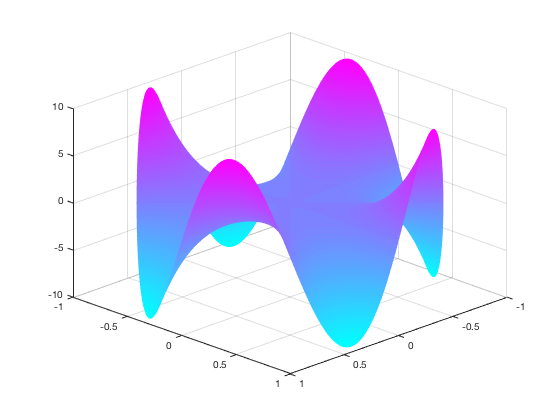
\includegraphics[width=5cm]{images/swing_function_plot.png}
  \caption{$u(x)$}%{Numerically solved solution}
  \label{fig:swingPlot}
\end{figure}


Equations can also be labeled
\begin{equation}
	\pi = \mathrm{e}^{i\cdot\phi}
	\label{eq:equation1}
\end{equation}


And later referenced. Even in subfigures.
\begin{figure}[!htb]
  \centering
  \begin{subfigure}[b]{0.3\textwidth}
    \centering
  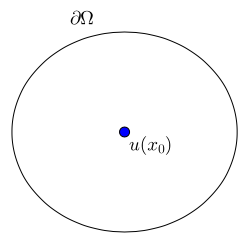
\includegraphics[width=\textwidth]{images/CircCenter}
  \caption{Equation \ref{eq:equation1}}\label{fig:circcenter}
\end{subfigure}
\hfill
  \begin{subfigure}[b]{0.3\textwidth}
    \centering
  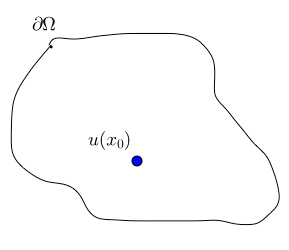
\includegraphics[width=\textwidth]{images/GeneralOffset}
  \label{fig:generaloffset}
  \caption{Equation \ref{eq:equation1}}
\end{subfigure}
\end{figure}
\section{Including code}

Code can be using the package
\href{https://www.sharelatex.com/learn/Code\_Highlighting\_with\_minted}{Minted}.

An exaple of which of can be found below (see Source Code \ref{lst:nice_listing})
\begin{listing}
	%the language syntax can be declared here.
	\begin{minted}{python} 
	import numpy as np
	
	def incmatrix(genl1,genl2):
	    m = len(genl1)
	    n = len(genl2)
	    M = None #to become the incidence matrix
	    VT = np.zeros((n*m,1), int)  #dummy variable
	
	    #compute the bitwise xor matrix
	    M1 = bitxormatrix(genl1)
	    M2 = np.triu(bitxormatrix(genl2),1)
	
	    for i in range(m-1):
	        for j in range(i+1, m):
	            [r,c] = np.where(M2 == M1[i,j])
	            for k in range(len(r)):
	                VT[(i)*n + r[k]] = 1;
	                VT[(i)*n + c[k]] = 1;
	                VT[(j)*n + r[k]] = 1;
	                VT[(j)*n + c[k]] = 1;
	
	                if M is None:
	                    M = np.copy(VT)
	                else:
	                    M = np.concatenate((M, VT), 1)
	
	                VT = np.zeros((n*m,1), int)
	
	    return M
	\end{minted}

  \caption{My nice listing}
  \label{lst:nice_listing}
\end{listing}


%
%% ---------------------------------------------------------------------------
%%
%% Thesis content: What did you do?
%%
%%% ---------------------------------------------------------------------------
\part[Body: What was done for the thesis]{Body: What Was Done for the Thesis}
\label{part:body}

%% ---------------------------------------------------------------------------
%%
%% Results and Conclusion
%%
%% ---------------------------------------------------------------------------
\part[Results and Conclusion]{Results and Conclusion}
\label{part:resultsAndConclusion}


% ---------------------------------------------------------------------------
%
% Appendix
%
% ---------------------------------------------------------------------------
\part*{Appendix}
\addcontentsline{toc}{part}{Appendix}

\appendix %---------------------------------------

% !TEX root = ../main.tex
\chapter{Detailed Descriptions}
%\section{Detailed Validation Results}
\label{chapter:DetailedDescriptions}\label{appendix}
%\inputminted{c++}{../../src/wos_native.cuh}
\newpage



 \clearemptydoublepage

 \printglossaries

 \addcontentsline{toc}{chapter}{Bibliography}
 \bibliography{bibliography/literature}

\end{document}
